
\section{Interval of Convergence}

With power series, be warned that not every infinite series will converge for all values of $x$. 

\begin{exercise}{A Convergent Series \Coffeecup}
Let us consider what happens when we evaluate the power series $$\cos(x)=1-\frac{1}{2!}x^2+\frac{1}{4!}x^4-\frac{1}{6!}x^6+\frac{1}{8!}x^8-\cdots  $$ at $x=1$.

We obtain the claim that $\cos(1)=1-\frac{1}{2!}+\frac{1}{4!}-\frac{1}{6!}+\frac{1}{8!}-\cdots$.  Let us test this numerically, remembering that an infinite series is really just a limit of partial sums.  Calculate decimal representations of the partial sums below.
\begin{center}
\begin{tabular}{|c|c|}\hline
Partial Sum & Decimal Approximation \\ \hline
$1$ & \\
$1-\frac{1}{2!}$ & \\
$1-\frac{1}{2!}+\frac{1}{4!}$ & \\
$1-\frac{1}{2!}+\frac{1}{4!}-\frac{1}{6!}$ & \\
$1-\frac{1}{2!}+\frac{1}{4!}-\frac{1}{6!}+\frac{1}{8!}$ & \\ \hline
\end{tabular}
\end{center}
Does it appear that the partial sums are converging to the true value of $\cos(1)$? \vspace*{1in}

\end{exercise}

\begin{exercise}{A Not-So-Convergent Series \Coffeecup}
Let us consider what happens when we evaluate the power series $$\ln(x)=(x-1)-\frac{1}{2}(x-1)^2+\frac{1}{3}(x-1)^3-\frac{1}{4}(x-1)^4+\frac{1}{5}(x-1)^5-\cdots  $$ at $x=3$.

We obtain the claim that $\ln(3)=2-\frac{1}{2}2^2+\frac{1}{3}2^3-\frac{1}{4}2^4+\frac{1}{5}2^5-\cdots $.  Let us again test this numerically, remembering that an infinite series is really just a limit of partial sums.  Calculate decimal representations of the partial sums below.
\begin{center}
\begin{tabular}{|c|c|}\hline
Partial Sum & Decimal Approximation \\ \hline
$2$ & \\
$2-\frac{1}{2}2^2$ & \\
$2-\frac{1}{2}2^2+\frac{1}{3}2^3$ & \\
$2-\frac{1}{2}2^2+\frac{1}{3}2^3-\frac{1}{4}2^4$ & \\
$2-\frac{1}{2}2^2+\frac{1}{3}2^3-\frac{1}{4}2^4+\frac{1}{5}2^5$ & \\ \hline
\end{tabular}
\end{center}
Does it appear that the partial sums are converging to the true value of $\ln(3)$? \vspace*{1in}

\end{exercise}

\subsection{\interval{Definition} of \powerseries{IOC}}

As you can see, power series expansions may be valid for some values of $x$ but not others.  The set of all the ``good'' $x$-values is called the interval of convergence.

\begin{definition}{Interval of Convergence}
Given a power series, the set of all $x$ values for which the infinite sum converges is called the \emph{interval of convergence} (IOC).  The midpoint of the interval is called the \emph{center} of the IOC and the distance from the center to endpoints is called the \emph{radius}. 
\end{definition}

On the interior of the interval, the power series will not only be convergent, but it will be absolutely convergent. This is of enormous convenience, because it means we are free to rearrange terms and do algebra as we like with our power series.

The fact that such a set is always an interval (as opposed to say just scattered points or a union of two disjoint intervals) is not obvious, but it turns out to be true.  To find the interval of convergence, it is typically easiest to use the Ratio Test.  Since power series always have powers of $x$, these will cancel nicely when we apply the Ratio Test.

\begin{example}{\ratiotest{Interval of Convergence} for Cosine}
Consider again our power series 
$$ \cos(x)=\sum_{n=0}^\infty (-1)^{n}\frac{1}{\left(2n\right)!}x^{2n}$$

Let us apply the Ratio Test to this series.  Our goal is to get the absolute value of the ratios of consecutive terms to be less than 1, in which case we are certain the series converges.

\begin{align*}
\lim_{n \rightarrow \infty}\left| \frac{a_{n+1}}{a_n} \right| &=\lim_{n \rightarrow \infty} \left|\frac{(-1)^{n+1}\frac{1}{\left(2(n+1)\right)!}x^{2(n+1)}}{(-1)^{n}\frac{1}{\left(2n\right)!}x^{2n}} \right| \\
 &=\lim_{n \rightarrow \infty} \left|\frac{x^{2n+2}\left(2n\right)!}{\left(2n+2)\right)!x^{2n}} \right| \\
 &=\lim_{n \rightarrow \infty} \left|\frac{x^{2}\left(2n\right)\left(2n-1\right)\cdots 3\cdot 2 \cdot 1}{\left(2n+2\right)\left(2n+1\right)\left(2n\right)\left(2n-1\right)\left(2n-2\right)\cdots 3\cdot 2 \cdot 1} \right| \\
 &=\lim_{n \rightarrow \infty} \left|\frac{x^{2}}{\left(2n+2\right)\left(2n+1\right)} \right| \\
 &=\left|x^2 \right| \lim_{n \rightarrow \infty} \left|\frac{1}{\left(2n+2\right)\left(2n+1\right)} \right| \\
 &=0\left|x^2 \right| \\
 &=0
\end{align*}
The ratio of consecutive terms, being zero, is always strictly less than one no matter what $x$ is.  Since it converges for every $x$ value, the interval of convergence is $(-\infty, \infty)$.
\end{example}

\begin{exercise}{Careful with Algebra! \Coffeecup}
Annotate each line above. Provide a short phrase indicating the reason each simplification was valid.
\end{exercise}

\begin{exercise}{IOC for Natural Log \Coffeecup \Coffeecup \Coffeecup}
Repeat the process above for the series $$ \ln(x)=\sum_{n=1}^\infty (-1)^{n+1}\frac{1}{n}(x-1)^{n}$$

For what $x$-values is the limit of ratios of consecutive terms less than one?

\vspace*{3in}

\end{exercise}

Notice in the above example, if $x=2$ or $x=0$, the limit of ratios of consecutive terms is equal to 1.  This is the case in which the ratio test gives us no information.  Thus, we must test these series for convergence separately.  We can use any of the tests from Section \ref{conv}.   

\begin{exercise}{Checking \interval{Endpoints} \Coffeecup \Coffeecup }
\begin{itemize}
\item Set $x=2$ in the series $\sum_{n=1}^\infty (-1)^{n+1}\frac{1}{n}(x-1)^{n}$ and test it for convergence/divergence.
\vspace*{1in}
\item Set $x=0$ in the series $\sum_{n=1}^\infty (-1)^{n+1}\frac{1}{n}(x-1)^{n}$ and test it for convergence/divergence.
\vspace*{1in}
\item Explain why the interval of convergence for $\ln(x)=\sum_{n=1}^\infty (-1)^{n+1}\frac{1}{n}(x-1)^{n}$ is $(0,2]$.
\vspace*{1in}
\end{itemize}
\end{exercise}

\subsection{Looking at IOC Graphically}

So far we found two IOC's.  Our series for cosine had IOC $\left(-\infty,\infty\right)$.  Our series for the natural logarithm had IOC $\left(0,2\right]$.  Let us compare these situations graphically!

\begin{exercise}{I See the IOC \Coffeecup \Coffeecup}
\begin{itemize}
\item Sketch the graph of cosine, and on the same axes plot the graphs of $P_n(x)$ for $n=0,1,2,3,4,5$, and 6.  You may use a CAS to help come up with the graphs of the polynomials.
\begin{center}
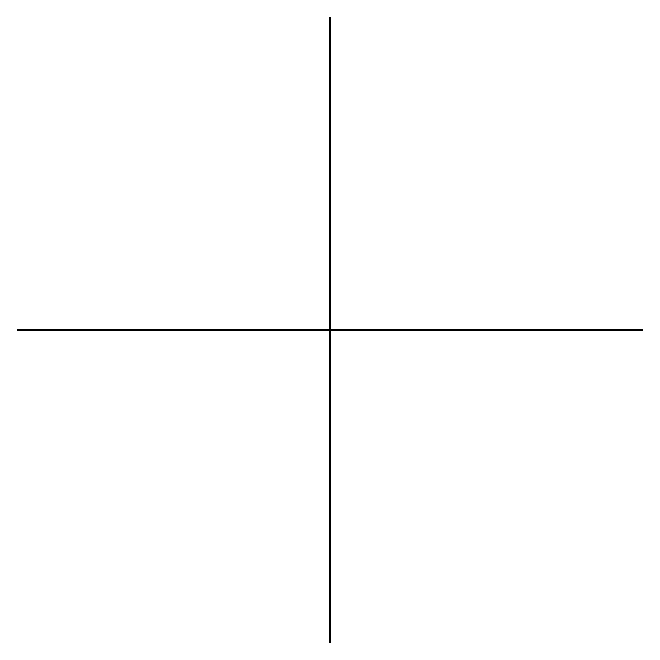
\includegraphics[scale=0.7]{quadall}
\end{center}
\item Sketch the graph of natural log, and on the same axes plot the graphs of $P_n(x)$ for $n=0,1,2,3,4,5$, and 6.  You may use a CAS to help come up with the graphs of the polynomials.
\begin{center}
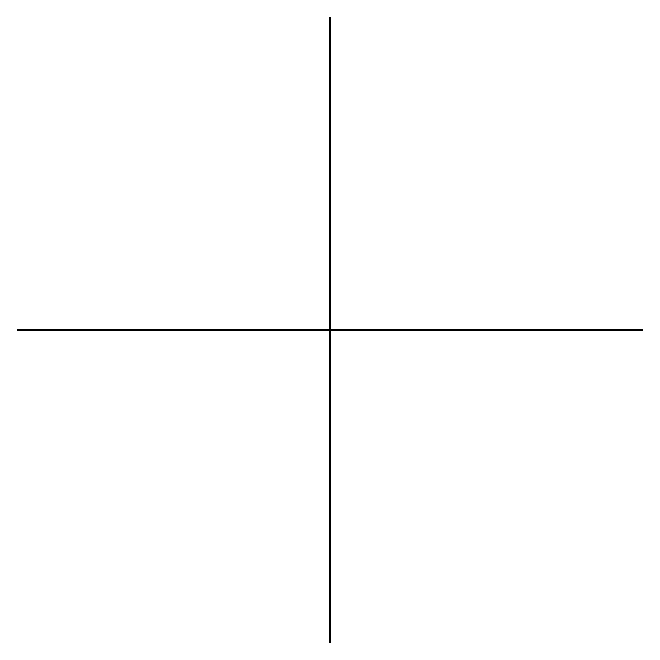
\includegraphics[scale=0.7]{quadall}
\end{center}
\item What feature of those graphs shows you the IOC? Explain!
\vspace*{1in}
\end{itemize}
\end{exercise}
